\section{Background :some backgrounds goes here, from the definition of model
formally, what is ATG, what is meta-model, What is State-based lenses, what is delta-base, 
what is Graph Grammer, Synchronization Properties : Correctness, Completeness, Hipocraticnes, Heridatiry and .... }

By \textbf {Synchronization}  we mean reconstructing the {\em Relation} between two {\em Models.} These two models already might have been in a consistent state, i.e. are related by R, or might be newly created models which consistency was not established between them yet. Models formally can be represented as an Attributed Types graph \cite{Ehrig:2004:FundementalATG, book:Ehrig2010}.  We are going to define some basic definitions regarding the formal foundation of Models in the following. These definition are adapted from \cite{book:Ehrig2010, Ehrig:2004:ATGFundemental}

\subsection{Model as an Typed Attributed Graph}
In general a Model can be represented as a Graph which consist of a nodes and edges connecting these nodes. e.g. a Class diagram in UML is a graph with classes as a node and the associations between the classes as a node. Since we need a richer structure than a simple graph we need to extend the formality of a graph to make it possible to capture further values annotated to the nodes and edges, Hence Attributed Graphs are introduced. Attributed graph are like ordinary graph extended in a way that for every {\em Node} and {\em Edge}, it is possible to introduced a Data called  {\em Attribute} and bind that by an edge called {\em Attribute Edge} to corresponding Nodes and Edges. So, first we need to extend the concept of regular graph to make it possible for the edges to have outgoing edges like nodes. This extended version of graphs is called {\em E-Graph} and introduced in the following.


%:Key Def1(E-graph G)
\begin{ProposalDef}
An \textbf{E-graph G} is defined as $G=(V_G,E_G, V_D, E_{NA},E_{EA} ,(source_j$ $,target_j)_{j \in \{G,NA,EA\}) }$
\begin{itemize}
	\item $(V_G,E_G,source_G,target_G)$ constitutes a regular Graph with $V_G$ as Nodes, $E_G$ as Edges and $source_G$ and $target_G$ as source and target functions  respectively.
	\item $V_D$ is a Data Nodes
	\item $E_{NA}$ and $E_{EA}$ are called Node Attributes and Edges Attributes, which are connecting respectively $V_G$  and $E_G$ to $V_D$. 
	\item source and target functions are defined as below:
	\begin{itemize}
		\item $source_G : E_G \rightarrow V_G$, $targetG : E_G \rightarrow V_G$;
		\item $source_{NA} : E_{NA} \rightarrow V_G$, $target_{NA}: E_{NA} \rightarrow V_D$;
		\item $source_{EA} : E_{EA} \rightarrow E_G$, $target_{EA}: E_{EA} \rightarrow V_D$;
	\end{itemize}
\end{itemize}

\end{ProposalDef}

%:Key Def2(morphism between E-graphs)
\begin{ProposalDef}

\textbf{morphism between E-graphs} $G^1$ and $G^2$ with 
$G^k = (V_G^k, V_D^k, E_G^k, E_{NA}^k$ $,E_{EA}^k, (source_j^k, target_j^k)_{j \in \{ G, NA, EA \}})$ for $k = 1, 2$ is defined as $f:G^1 \rightarrow G^2$ which is a tuple $(f_{V_G},f_{V_D},f_{E_G},f_{E_{NA}},f_{E_{EA}})$ 
with $f_{V_i} : V_i^1 \rightarrow V_i^2$ and  $f_{E_j} : E_j^1 \rightarrow E_j^2$ for $i \in \{G,D\}$, $j \in \{G,NA,EA\}$ such that $f$ commutes with all source and target functions, for example $f_{V_G}  \circ source_G^1= source_G^2 \circ f_{E_G}$

\end{ProposalDef}

%:Key Def3(Category EGraphs)
\begin{ProposalDef}
E-graphs and E-graph morphisms form the \textbf{Category EGraphs}.
\end{ProposalDef}

 {\em Attributed Graphs} are Graphs that is accompanied by a Data Algebra in a sense that the Data Nodes are taken from the subset of algebra {\em Carrier sets}. To be more precise, we first distinguish a subset of a Carrier set of an algebra and consider the contents of each member in this subset as a {\em Data Node}. In graphical illustration of the Attributed Typed Graph we ignore those {\em Data Nodes} that are not reachable from the underlying Graph Nodes and Edges. See an example in \cite{book:Ehrig2010} for more details.
  
%:Key Def4 (Att Graph Def)
\begin{ProposalDef}
Let $D_{SIG} = (S_D,OP_D)$ be a data signature with attribute value sorts $S_D$ and operations $OP_D$ and take $S'_D \subseteq S_D$. An \textbf{Attributed Graph(AG)} $AG = (G,D)$ consists of an E-graph $G$ together with a $D_{SIG}$-algebra $D$ such that $V_D$ is disjoint union of the selected carrier sets, i.e. $V_D=\overset{\centerdot}{\cup}_{s \in S'_D} D_s$ where $D_s$ is coresponding carrier set of s.
\end{ProposalDef}

%:Key Def5 (Att Graph Morphism )
\begin{ProposalDef}
an \textbf{Attributed Graph Morphism}  $f : AG^1 \rightarrow AG^2$ for two AG graphs $AG^1=(G^1,D^1)$ and $AG^2 = (G^2,D^2)$ is a pair $f=(f_G,f_D)$ with an E-graph morphism $f_G : G^1 \rightarrow G^2$ and an algebra homomorphism $f_D : D^1 \rightarrow D^2$ such that diagram (1) commutes for all $s \in S'_D$, where vertical arrows are inclusions:

\begin{figure}[ht!]
\centering
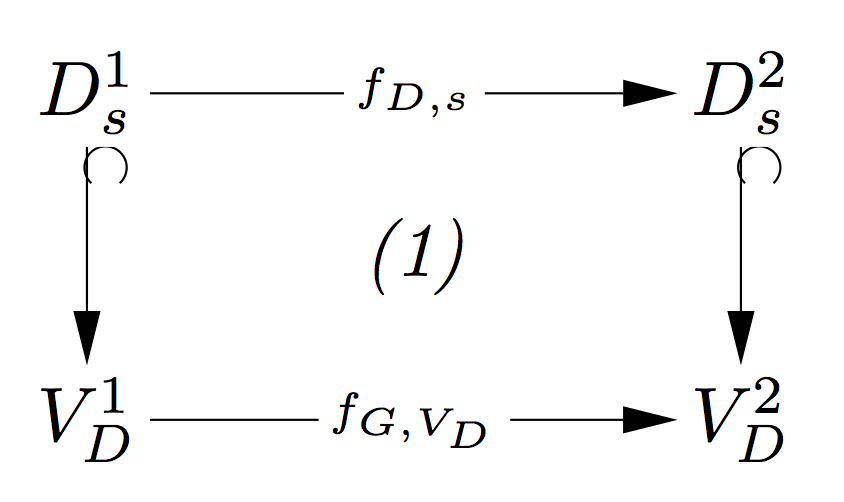
\includegraphics[width=60mm]{images/AGmorphism.png}
%\caption{AG }
\label{AG morphism}
\end{figure}

\end{ProposalDef}

For defining the Typed attributed Graph we need to first define the concept of final $D_{sig}$-algebra for a given algebra. final $D_{sig}$-algebra for an algebra is mapping somehow the name of the sort as a set to the sort as its interpretation. So cardinality of the interpreted sorts would be 1 for all of them. It maps the constant symbol of sort $S_i$, to the singleton member of corresponding carrier set $Z_{S_i}$, and following that, interpret the result of a function application on carrier set to the corresponding singleton member of the result sort.  
%:Key Def6 (final D_sig-Algebra)
\begin{ProposalDef}
Given a signature $SIG = (S, OP)$ , the \textbf{final $SIG$-algebra Z} is defined by $Z=(S_z, C_z, OP_z)$ where:

\begin{itemize}
	%\item $S_z = D_k$ where  $D_k=\{k\}$ for each sort $k \in S$;
	\item $S_z = D_s$ where  $D_s=\{s\}$ for each sort $s \in S$;
	%	\item $C_z = s \in Z_s$  for a constant symbol $c_s: \rightarrow s \in OP$;
	\item $C_z = k \in D_s$  for a constant symbol $c_s: \rightarrow s \in OP$;
	%\item $op^I : \{s_1\} \ldots  \{s_n\} \rightarrow \{s\} : (s_1 ... s_n) \mapsto s$ for each operation symbol $op:s_1 ... s_n \rightarrow s \in OP$
	\item $OP_z : \{s_1\} \ldots  \{s_n\} \rightarrow \{s\} : (s_1 ... s_n) \mapsto s$ for each operation symbol
$op:s_1 ... s_n \rightarrow s \in OP$
 \end{itemize}

\end{ProposalDef}


%%:Key Def6 (Typed Att Graph)
%\begin{ProposalDef}
%an \textbf{Attributed Graph Morphism}  $f : AG^1 \rightarrow AG^2$ for two AG graphs $AG^1=(G^1,D^1)$ and $AG^2 = (G^2,D^2)$ is a pair $f=(f_G,f_D)$ with an E-graph morphism $f_G : G^1 \rightarrow G^2$ and an algebra homomorphism $f_D : D^1 \rightarrow D^2$ such that diagram (1) commutes for all $s \in S'_D$, where vertical arrows are inclusions:
%
%\begin{figure}[ht!]
%\centering
%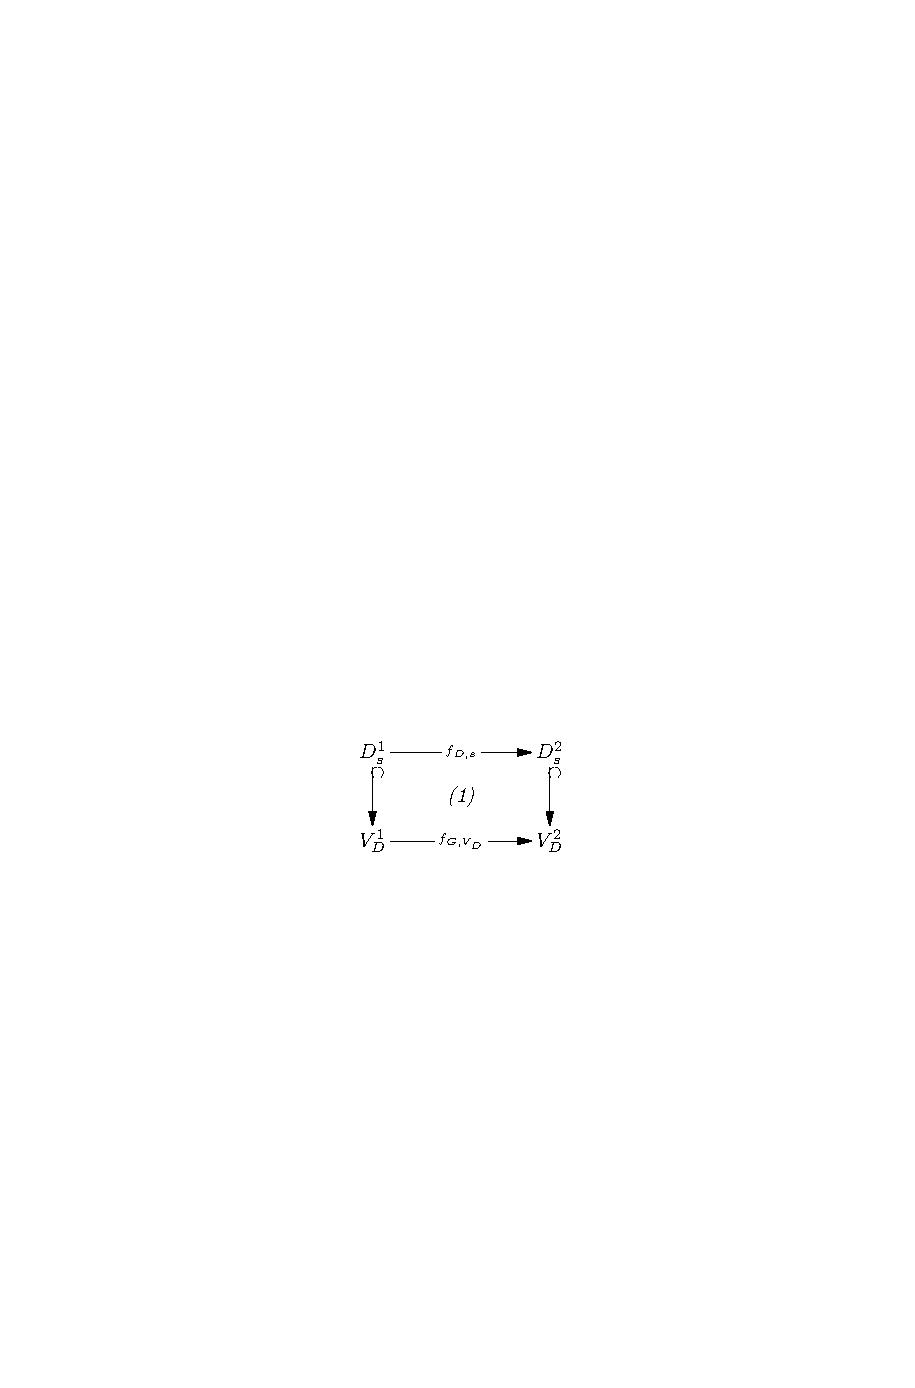
\includegraphics[width=60mm]{images/AG-morphism}
%%\caption{AG }
%\label{AG morphism}
%\end{figure}
%
%\end{ProposalDef}

%:Key Def (Attributed Type Graph(ATG))
\begin{ProposalDef}
Given a signature $SIG = (S, OP)$ , an \textbf{Attributed Type Graph(ATG)} is an attributed graph $ATG=(TG,Z)$ where Z is the final $SIG$-algebra. 
\end{ProposalDef}

So for having an Attributed Type Graph as a Type of another Attributed Graph, we need to somehow specify the typing of the 
Attributed Graph Data Structure(Data Algebra) too. That is why we need to define a final $Sig$-algebra. Typing of the Attributed Graph Data Structure is represented by the final $SIG$-algebra of the corresponding Data Signature. In the following we define Typed Attributed Graph (TAG).

%:Key Def (Typed Attributed Graph)
\begin{ProposalDef}
\label{Def:TAG}
A \textbf{Typed Attributed Graph(TAG)} over $ATG$ is defined as $(AG, t)$  where $AG$ is an attributed graph and $t$ is an  attributed graph morphism from $AG$ to $ATG$
\end{ProposalDef}


Please observe that the data-signature of of the Attributed Type Graph and Typed Attributed Graphs, Typed over that would be the same, as the definitions above implies.

\begin{ProposalDef}
A \textbf{TAG morphism} between $TAG^1=(AG^1,t^1)$ and  $TAG^2=(AG^2,t^2)$ i.e. $f: TAG^1 \rightarrow TAG^2$ is an Attibuted Graph Morphism(AGT morphism) $f: AG^1 \rightarrow AG^2$ such that $t^2 \circ f=t^1$:
\end{ProposalDef}

\begin{figure}[ht!]
\centering
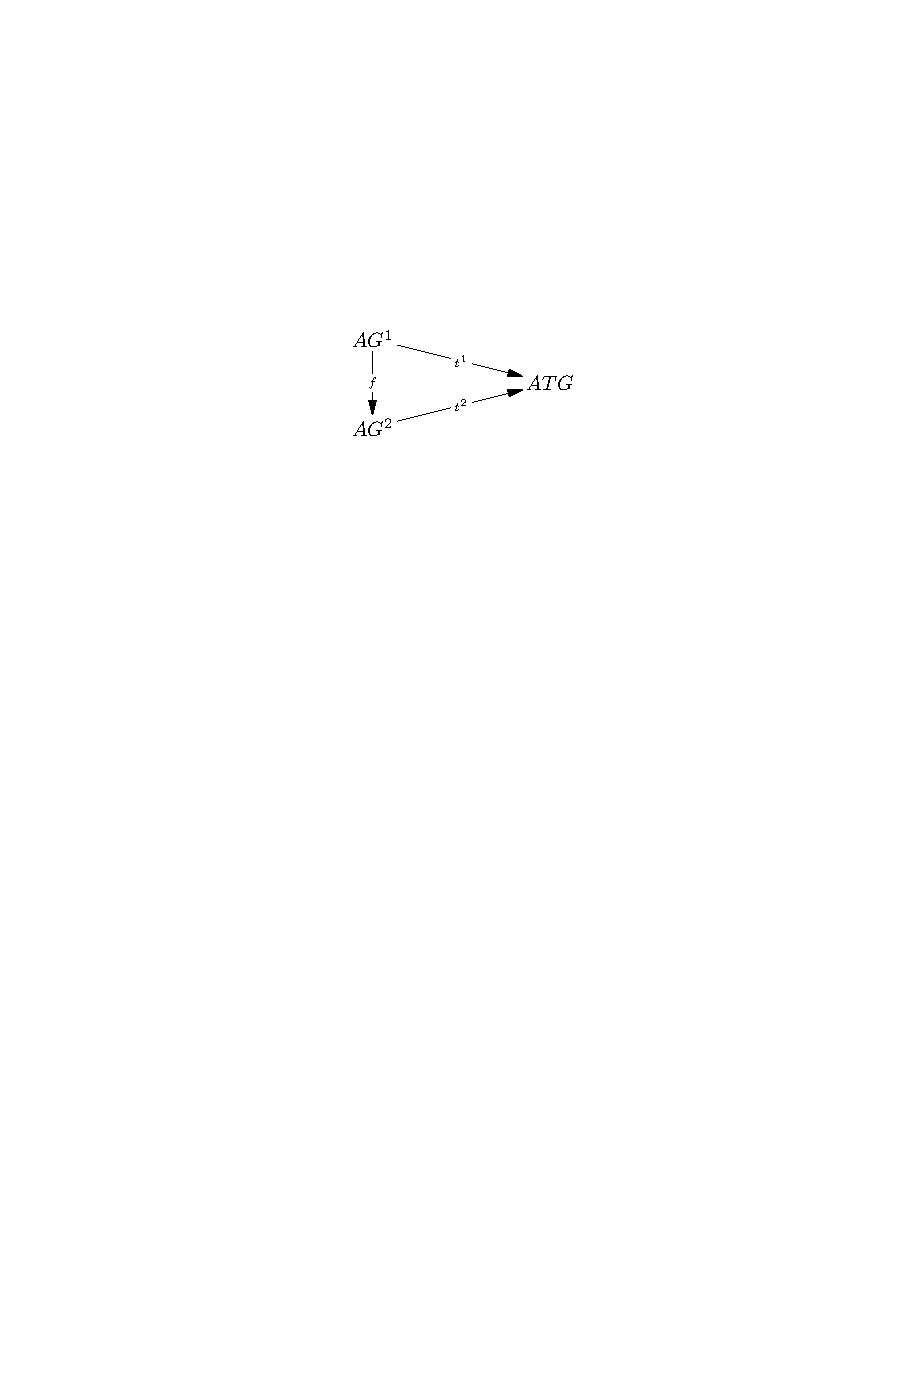
\includegraphics[width=60mm]{images/TAG-morphism}
%\caption{AG }
\label{AG morphism}
\end{figure}

In terminology of the Software Engineering, {\em Models} are equal to {\em Typed Attributed Graphs} and {\em Meta-Models} are equal to {\em Attributed Type Graphs}. This can be extended to more than one level, while meta-meta-model would be Attributed Type Graph for Attributed Type Graph of its beneath level as a Type. We should observe that all the {\em Entities} (Including Models, Meta-Models and Meta-Meta-Models) are Attributed Graphs, and the Data-signature of the connected {\em entities} by typing association(Typing Mapping) would be the same. In another word data-signature of the Model, Meta-Model and Meta-Meta-Model, all, would be the same.